\chapter{Methods and Background}
In this chapter we formulate our problem background and the history of machine learning and PET images in literature. After setting us some goals and motivation we will introduce in brevity the Machine Learning techniques we propose to use.  

\section{Background}
\label{sec:background}
In Chapter.~\ref{chapter:subjects_perprocessing} the PET data is processed and made ready to use. In this section we look into the problem background, formulate mathematical frameworks to base our analysis and look into the history of Machine Learning with respect to \FDGPET~and discuss it as a reliable biomarker.

\subsection{Problem Background}
ADNI2 is divided into five cohorts namely (AD), (LMCI), (EMCI), (SMC) and (CN) (Table.~\ref{fig:participant_stages}). The overall goal of ADNI is to validate biomarkers for use in Alzheimer’s disease clincal treatment trials. ADNI is not a population based study and enrolls selected populations who may be used in future treatment trials. Therefore the results from ADNI may not be generalizable to other populations. Dementia, one of the most feared associates of increasing longevity, represents a pressing public health problem and major research priority. The ADNI study is a major step toward the early diagnosis and detection of (AD). Increasing knowledge over the last years about the pathomechanisms involved in AD allow for the development of specific treatment strategies aimed at slowing down or even preventing neuronal death in AD.

There is a sense of urgency in find imaging techniques and biomarkers. It is required that:

%% reason for choosing PET

\begin{itemize}
	\item AD be classified from normal control with high accuracy because non-AD dementias would not benefit from an AD-specific treatment
  	\item AD progression be tracked and distinguished from lower levels of dementia (EMCI, LMCI \& SMC in case of ADNI2) when an intervention would be most effective.
  	\item The treatment efficacy be reliably and meaningfully monitored 
\end{itemize}

In the report by \citep*{mueller2005ways} there is a mention that no one biomarker exists yet that fulfills all the above requirements. Yet there is increasing evidence that a combination of currently existing neuroimaging techniques and different biomarkers can provide important complementary information and thus contribute to a more accurate and earlier diagnosis of AD. Leading us to investigate the demographic feature.  

We design six experiments (1). AD vs. CU (2). AD vs. EMCI (3). AD vs. LMCI (4). CU vs. EMCI (5). CU vs. LMCI (6). EMCI vs. LMCI. The objective here is to independently study the inter-cohort relationships in hope of learning more about the class separation in AD clinical group.

\subsection{History of M.L. and FDG-PET}
A \FDGPET~ scan uses a small amount of fluorodeoxyglucose (FDG) tracer ergo ``FDG-PET'' to show differences between healthy tissue and diseased tissue. The radioactive tracer will take 30 to 90 minutes for it to travel through the body. In previous studies FDG-PET is described as a
“neuronal injury” biomarker in AD~\citep{ishii2002clinical,ishii2014pet}.

In the report ``PET approach for dementia diagnosis''\cite{ishii2014pet} states that FDG-PET generally has a higher accuracy than MR imaging for diagnosis of early AD and for predicting rapid conversion for mild cognitive impairment (MCI) to AD. This is corroborated by Fig.~\ref{fig:biomarker} where the strength of the curve is maximum for amyloid-PET during the early stages. For statistical voxel based analysis the researches have proposed for automatic diagnosis the t-sum method of calculating the total t-values in a region-of-interest template by using the Statistical Parametric Mapping (SPM) program. 
In other works \citep*{rabinovici2011amyloid} FDG-PET has been compared against amyloid ligand Pittsburgh
compound B (PiB-PET) and has been used to differentiate between  frontotemporal lobar degeneration (FTLD) and AD. The study concluded that PiB and FDG showed similar accuracy in discriminating AD and FTLD. 

%% edit t values and z score correction
For 3D PET scans ``Z-score'' images are used to represent the active parts of the brain it will show all pixels with values below the lower threshold in blue, and pixels above the upper threshold in red~\citep{ishii2014pet}. PET scans have also been analyzed by utilizing adjusted $T$ statistics and an automated voxel-based procedure~\citep{herholz2002discrimination} and Machine Learning algorithms to address the high dimensionality of the statistical maps~\citep{illan201118}~\citep{higdon2004comparison}. Recently minor cognitive impairment (MCI) in \FDGPET ~has been classified by a brain regional sensitivity mapping method based on summated index (Total Z score) by utilizing the sensitivity-distribution maps~\citep{kakimoto2011new}. In other contemporary works a region of interest (ROI) mask is used to extract features and use incomplete random forest-robust support vector machine to perform classification~\citep{lu2017early}. In previous work within our lab MRI images were classified using surface measures of ventricular enlargement and sparse coding then applied on the 2D-patch features~\citep*{zhang2016hyperbolic,zhang2016applying} with $ 96.7 \% $ accuracy. These images were functional MRIs and the features were a combination of surface statistics, we build our idea on a similar model we fist design a empirical machine learning based model. Using three dimensional patches (i.e., small sub volumes of the image defined as three-dimensional [3D] cubes) we extract information. A very similar 3D patch based feature selection is described in \citep{coupe2011patch}, In  this work, voxels  with  similar  surrounding  neighborhoods  are  considered  to  belong  to  the  same  structure and thus are used to estimate the final label. Our data is also along the same lines. 

\subsection{Biomarker}
The Figure~\ref{fig:biomarker} depicts the biomarkers as indicator of dementia. The curve indicates the strength of the biomarker with respect to dementia state. The common imaging and assessment modalities are:
\begin{enumerate}
	\item Amyloid beta imaging modality detected in CSF and PET-Amyloid.
	\item Neuro-degeneration detected by \FDGPET.
	\item Brain atrophy and neuron loss measured with MRI.
	\item Memory loss measured by cognitive assessment
	\item General cognitive decline measured by cognitive assessment 
\end{enumerate}

1-3 biomarkers can be observed before the diagnosis of dementia, and our data is of the second type measuring the neuronic activity at a given time. \FDGPET~ scan is a 30 min procedure and requires the patient to stay still in a dark room. The varition in neuronic activity at a time if any is accounted as outliers and it depends on the chosen algorithms to handle outliers. The graph in Fig.~\ref{fig:biomarker} gives us an insight into how out classification would perform given the biomarker as \FDGPET. AD vs. CU would be easily separable, groups like EMCI vs. LMCI who have close separation in progression may be the most difficult to classify and early changes in disease progression should have a strong separation but not as strong as in case of AD vs. CU.        

\begin{figure}[h]
	\centering
	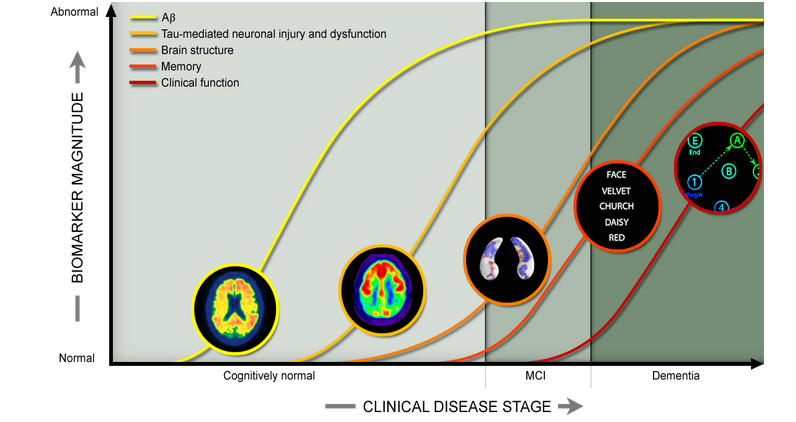
\includegraphics[width=\linewidth]{figures/biomarker}
	\caption[Biomarkers vs. dementia]{Biomarkers vs. dementia in symptomatic stages of AD. The curves to right (yellow(PET), melon-orange (PET)) have strong early slopes indicating early class separation, curves to the right (orange (MRI), red (assessments)) have strong slopes in later stages.}
	\label{fig:biomarker}
\end{figure}


\section{Methods}
\label{sec:theoritical_background}

In this section, we briefly introduce the most relevant theoretical background in Sparse Coding, Dimensionality Reduction, Max-Pooling and Adaptive Boosting (Adaboost). The underlying algorithm are described in detail in Chapter.~\ref{chapter:algorithm}.

\subsection{Dictionary Learning and Sparse Coding} 
Sparse coding is the modeling of data vectors as sparse linear combinations of basis elements it is widely used in machine learning, neuroscience, signal processing, and statistics. From the input image data, sparse coding learns an over-complete set of basis vectors (dictionary), which have been used to represent data efficiently~\citep{tibshirani1996regression,friedman2008sparse}. To learn local imaging features, image patches are usually selected to form dictionaries. We first generate a 10 $\times$ 10 $\times$ 10 window on the 3D scan to obtain a collection of small image patch with constant overlap. We used the technique of dictionary learning and sparse coding to learn meaningful features based on stochastic approximations, which scales up gracefully to large datasets with millions of training samples. Stochastic Coordinate Coding (SCC)~\citep{lin2014stochastic} was adopted in our work for dictionary construction because of its computational efficiency.

Given a data set $\mathbf{X} = (x_1 \dots x_n)$ of image patches, each image patch is a {\em p}-dimensional vector i.e., $ x_i \in \mathbb{R}^{p} $, $ i = 1, \dots, n $. Specifically, suppose there are \emph{m} atoms $ \mathbf{d_j} \in \mathbb{R}, j = 1,\dots,m $, where the number of atoms is usually much smaller than the number of image patch {\em p}. Each patch can be represented as $ \mathbf{x_i} =  \sum^m_{j=1} z_{i,j}d_j $. In this way, the {\em p}-dimensional vector $ \mathbf{x_i} $ is represented by an m-dimensional vector $  \mathbf{z_i} = (z_{i,1},\dots,z_{1,m})^T $ which means the learned feature vector $ \mathbf{x_i} $ is a sparse vector. We can then formulate the following optimization problem:

\begin{equation}\text{min} \,\, f_i(D,z_i) = \frac{1}{2}\|Dz_i - x_i\|^2 + \lambda\|z_i\|_1 \end{equation}

where $ \lambda $ is the regularization parameter, $ \|\,.\,\| $ is the Euclidean norm and $ \|z_i \|_1 = \sum^m_{j=1}|z_{i,j}| $. We can interpret the first term of the Eq(1) as a reconstruction term which tries to force the algorithm to provide a good  representation of $\mathbf{x}$. The second term of Eq(1) ensures the sparsity of the learned features $ \mathbf{z_i} $. $ D = (d_1,\dots,d_m) \in \mathbb{R}^{p \times m} $ is the dictionary. Given the whole dataset $\mathbf{X}$., the sparse coding problem is then given as follows:
\begin{equation}\underset{D \in B_m,\mathbf{z_1},\dots,\mathbf{z_m}}{\text{min}} \,\, \mathcal{F}(D,z_1,\dots,z_m) \equiv \frac{1}{n}\sum^n_{i = 1}f_i(D,z_i),\end{equation}

It is a non convex problem with respect to joint parameters in the dictionary  $\mathbf{D}$ and the sparse code $ \mathbf{Z} = \mathbf{z_1},\dots,\mathbf{z_m} $.However, it is a convex problem when either D or Z is fixed. When the dictionary is fixed, solving each sparse code $z_i$ is a Lasso problem. Because the PET scan feature dimension $m$ is much larger than than $n$, solving the Lasso problem is time consuming. On the other hand when the sparse codes are fixed, it will become a quadratic problem. Solving the sparse coding problem also requires a lot of time when dealing with large-scale data sets and a large-size dictionary. Thus we choose the stochastic coordinate coding(SCC) algorithm~\citep{lin2014stochastic}, which can dramatically reduce the computational costs of the sparse coding while keeping a comparable performance. The dictionary learning and sparse coding based on SCC algorithm may involve many rounds of iteration. One iteration is described in Fig.~\ref{fig:pipeline}(c). In many computer vision, medical imaging and bioinformatics applications~\citep{mairal2009online,zhang2010discriminative,lv2015modeling} dictionary learning and sparse coding leads to state-of-the-art results.

\subsection{Max-Pooling} 
State-of-the-art patch-based image representations involve a pooling operation that aggregates statistics computed from local descriptors. After obtaining features using convolution, we would next like to use them for classification. In theory, one could use all the extracted features with a classifier such as a softmax classifier, but this can be computationally challenging. We use max-pooling which summarizes the coded features over larger neighborhoods. To address this, first recall that we decided to obtain convolved features because images have the "stationarity" property, which implies that features that are useful in one region are also likely to be useful for other regions. Thus, to describe a large image, one natural approach is to aggregate statistics of these features at various locations. If one chooses the pooling regions to be contiguous areas in the image and only pools features generated from the same (replicated) hidden units. Then, these pooling units will then be translation invariant. This means that the same (pooled) feature will be active even when the image undergoes (small) translations. Translation-invariant features are often desirable; in many tasks (e.g., object detection, audio recognition), the label of the example (image) is the same even when the image is translated. For example, if you were to take an MNIST digit and translate it left or right, you would want your classifier to still accurately classify it as the same digit regardless of its final position. Standard pooling operations include sum- and max-pooling. Sum-pooling lacks discriminability because the resulting representation is strongly influenced by frequent yet often uninformative descriptors, but only weakly influenced by rare yet potentially highly-informative ones. Max-pooling equalizes the influence of frequent and rare descriptors but is only applicable to representations that rely on count statistics, such as the bag-of-visual-words (BOV) and its soft-and sparse-coding extensions. Fig. \ref{fig:maxpooling} shows the whole process of max pooling. On the left hand side, pooling layer down-samples the volume spatially, independently in each depth slice of the input volume. On the right hand side, it is the most common max pooling shown with a stride of 2.
\begin{centering}
	\begin{figure}
		\centering
		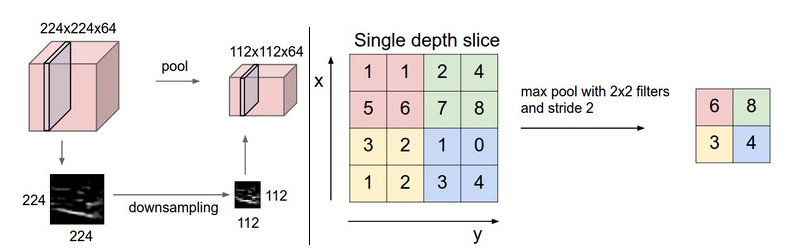
\includegraphics[width=\linewidth]{figures/maxpooling2.png}
		\caption[Maxpooling and Downsampeling.]{Pooling layer down-samples the volume spatially, independently in each depth slice of the input volume. Left: In this example, the input volume of size [256×256×16] is pooled with filter size 2; stride 2 into output volume of size [128×128×16]. Notice that the volume depth is preserved. Right: The most common down-sampling operation is max, giving rise to max-pooling, and here shown with a stride of 2, each max value is taken over 4 numbers (little 2×2 square).}
		\label{fig:maxpooling}
	\end{figure}
\end{centering}

\subsection{Dimension Reduction}
Feature extraction approaches project features into a new feature space with lower dimensionality and the new constructed features are usually combinations of original features. Examples of feature extraction techniques include Principle Component Analysis (PCA), Linear Discriminant Analysis (LDA) and Singular Value Decomposition(SVD). Feature extraction maps the original feature space to a new feature space with lower dimensions by combining the original feature space. In that context principle component analysis (PCA)~\citep{jolliffe2002principal} is a unsupervised machine learning algorithm widely used for dimensionality reduction. It used orthogonal transformations to convert a set of observations of possibly co-related values into a set of linearly uncorrelated variables called principle components. 

After selecting the patches and structuring our 3D data into ``sample $ \times $ features'', we would wish to analyze it summarizing its main characteristics. PCA is one of the most popular techniques for processing, compressing and visualising data. We use probabilistic PCA a variation of traditional PCA to reduce the dimensions of our selected features. Traditionally PCA's effectiveness is limited by its global linearity, to overcome that a combination of local linear PCA projections has been found to be able to capture data complexity efficiently. This model variant of PCA corresponds to the probability density unlike traditional PCA and enables it to combine PCA models~ \citep{tipping1999mixtures}. After reducing the dimensions of our dataset we will classify using AdaBoost. 


\begin{centering}
	\begin{figure}
		\centering
		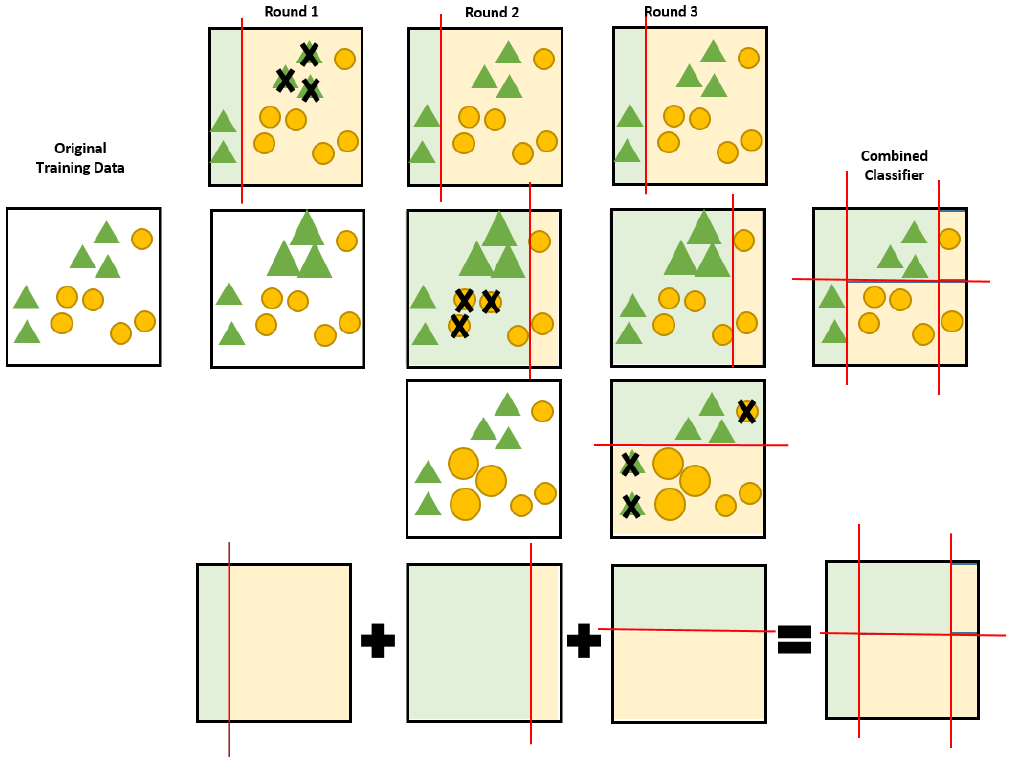
\includegraphics[width=\linewidth]{figures/adaboost.png}
		\caption[Illustration of the AdoBoost Algorithm.]{Illustration of the general idea of AdaBoost algorithm. The original training data is trained in three rounds. The first round is to create the first classifier, then the wrong classes will be given more weight and train in next round. In round 2, AdaBoost constructs a new classifier on the different weighted data. Similarly, it will give wrong classes higher weight and increase the probability of training in next round. Here, $ \times $ represents wrong classes. In the third round, AdaBoost learns a new classifier based on last round weighted data. In this figure, the bigger shape means more weight to be trained. Finally, AdaBoost combines all classifiers in three rounds (calculated in last line) into the final classifier.}
		\label{fig:adaboost}
	\end{figure}
\end{centering}

\subsection{AdaBoost}
A number of statistical classifiers have been proposed for brain biomarker research. Support vector machine and Adaptive Boosting are the most popular ones. Adaboost short for ``Abstract Boosting'' is an approach to machine learning based on the idea of creating a highly accurate prediction rule by combining many relative weak and inaccurate rules. The AdaBoost Algorithm~\citep{freund1996experiments} was the first practical boosting algorithm, and remains one of the most widely used and studied, with applications in numerous fields. Adaboost can achieve more accuracy than any individual member classifier with unstable classifier. It can be used in conjunction with many other types of learning algorithms to improve their performance. One of the main ideas of the algorithm is to maintain a distribution or set of weights over the training set.  Initially, all weights are set equally, but on each round, the weights of incorrectly classified examples are increased so that the weak learner is forced to focus on the hard examples in the training set. Fig. \ref{fig:adaboost} illustrates the general idea of the AdaBoost algorithm. The algorithm takes as input a training set $ (x_1,y_1), \dots , (x_m,y_m) $ where each $ x_i $ belongs to some domain or instance space $ X $, and each label $ y_i $ is in some label set $ Y $. For most of the discussion, we assume $ Y = \{-1, +1\} $. Adaboost calls a given weak or base learning  algorithm repeatedly in a series of rounds $ t = 1,\dots,T $. One of the main ideas of the algorithm is to maintain a distribution or set of weights over the training set. The weight of this distribution on training example $ i $ on round $ t $ is denoted as $ D_t(i) $. Initially, all weights are set equally , but on each round, the weights of incorrectly classified examples are increased so that the weak learner is forced to focus on the hard examples in the training sets.
The weak learner's job is to find a weak hypothesis $ h_t : X \to \{-1 ,+1\}$ appropriate for the distribution $ D_t $. The goodness of a weak hypothesis is measured by its error.
$$ \epsilon_t = Pr_{i \sim D_t}[h_t(x_i) \neq y_i] = \underset{i:h_t(x_i) \neq y_i}{\sum} D_t(i)  $$
Notice that the error is measured with respect to the distribution $ D_t $ on which the weak learner was trained. In practice, the weak learner may be an algorithm that can use the weights $ D_t $ on the training examples. Alternatively , when this is not possible, a subset of the training examples can be sampled according to $ D_t $, and these (unweighted) resampled examples can be used to train the weak learner~\cite{schapire2013explaining}

